%%% This is an example file for the Auburn University style options
%%%       aums.sty (Masters Thesis)
%%%       auphd.sty (Ph.D. Dissertation)
%%%       auhonors.sty (Honors Scholar)

%%%To use it, please edit the necessary options, title, author, date, year, keywords, advisor, professor, etc. 

\documentclass[12pt]{report}
%\usepackage{aums}       % For Master's papers
%\usepackage{auphd}     % For Ph.D.
\usepackage{auhonors}  % For honors college
\usepackage{ulem}       % underlining on style-page; see \normalem below
\usepackage{url}
\usepackage{tikz}
\usepackage{pgf}
\usepackage{tocloft}
\usepackage{sectsty}
\usepackage{indentfirst} %abstract indent para
\usepackage{wrapfig} %figures embedded in text
\usepackage{subcaption} %subfigures 
\usepackage{float} %"attach" figures to sections
\usepackage{titlesec} %making \section headers smaller
\usepackage{booktabs} %table styling
\usepackage{syntax} % CFG styling
\usepackage{listings} %both for code blocks
\usepackage{color}

\graphicspath{ {images/} }

\definecolor{dkgreen}{rgb}{0,0.6,0}
\definecolor{gray}{rgb}{0.5,0.5,0.5}
\definecolor{mauve}{rgb}{0.58,0,0.82}

\lstset{frame=tb,
  language=Python,
  aboveskip=0.0mm,
  belowskip=0.0mm,
  showstringspaces=false,
  columns=flexible,
  basicstyle=\linespread{1.25}\small\ttfamily,
  numbers=left,
  numberstyle=\tiny \color{gray},
  keywordstyle=\color{blue},
  commentstyle=\color{dkgreen},
  stringstyle=\color{mauve},
  breaklines=true,
  breakatwhitespace=true,
  tabsize=3
}

%%%%%Format rules: Normal margins are 1 in. If you need to print with 1.5in margins, uncomment the line below
\oddsidemargin0.5in \textwidth6in


\chapterfont{\centering \large}
\renewcommand{\cfttoctitlefont}{\normalsize \textbf}
\renewcommand{\cftloftitlefont}{\normalsize \textbf}
\renewcommand{\cftlottitlefont}{\normalsize \textbf}

\titleformat*{\section}{\normalsize}

% May want theorems numbered by chapter
\newtheorem{theorem}{Theorem}[chapter]


\begin{document}



\begin{titlepage}
    \begin{center}
        \vspace*{1cm}
        
        \Large
        \textbf{USING STATISTICAL DISTRIBUTIONS FOR GENERATING RANDOM TEST DATA}
        
        \vspace{3.5cm}
        
        \large
        by
        \linebreak
        JAMIE ZIMMERMAN
        
        \vspace{3.5cm}
        
        \vfill

        \normalsize
        A THESIS
        \vspace{1.5cm}
        \begin{singlespace}
        Presented to the Department of Computer and Information Science \\
        and the Robert D. Clark Honors College \\
        in partial fulfillment of the requirements for the degree of \\
        Bachelor of Science
        \end{singlespace}
        
        \vspace{0.8cm}
        June 2018
        
    \end{center}
\end{titlepage}



\begin{romanpages}      % roman-numbered pages 

%abstract
\thispagestyle{plain}
\begin{center}
%\large\textbf{An Abstract of the Thesis of}

%\vspace{.75cm}

\normalsize Jamie Zimmerman for the degree of Bachelor of Arts \\
in the Department of Computer and Information Science to be taken June 2018.

\vspace{2cm}


Title: Using Statistical Distributions to Generate Random Test Data

\vspace{1.5cm}

Approved: \hrulefill

Dr. Michal Young

\end{center}
Here is my abstract.
 \vfill

%acknowledge
\newpage
\thispagestyle{plain}
\begin{center}

\normalsize \textbf {Acknowledgements}
\end{center}


My acknowledgements to Michal, Hank, Rebecca, and others.

\newpage

\begin{center}
\tableofcontents
\end{center}

%materials
\thispagestyle{plain}

\newpage
\begin{center}

\textbf{List of Accompanying Materials}

\vspace{.5cm}

\begin{enumerate}
\item GenSequence: https://github.com/TestCreator/GenSequence \\
\item GenPairs: https://github.com/TestCreator/GenPairs
\end{enumerate}
\end{center}


%terms
\thispagestyle{plain}
\newpage
\begin{center}


\textbf{List of Terms}

\vspace{.5cm}

\begin{itemize}
\item []\textbf{SUT} - Software Under Test, the program to be tested
\item []\textbf{Production Rule} - a recursive rule that describes what the left-hand symbol could possibly be. For example, an A could be a B, denoted by A $\,\to\,$ B. Whenever an A is seen, one can choose to replace it with a B.
\item []\textbf{Test Vector} - A symbolic description of a test case, lacking exact data points but having an English language descriptor
\item []\textbf{Fault} - a misbehavior in a software program, also known as a bug. The behavior can vary from a program crash to an unexpected, nonsensical output
\item []\textbf{CSV file format} - a comma-separated value file that is viewable in Microsoft Excel
\end{itemize}
\end{center}

\newpage

\begin{center}
\listoffigures
\end{center}


\newpage
\begin{center}
\listoftables
\end{center}


\end{romanpages}        % All done with roman-numbered pages%

\normalem       % Make italics the default for \em%

\chapter{\normalsize Introduction}
%introduction

Software testing is a crucial part of systems that run our lives. Industries that rely on predicting consumer habit trends or dispatching taxi cars are terribly effected when their software fails to provide accurate results. The gravity of this trust is even greater in safety-critical programs controlling gas-leak shut off valves or anesthetic delivery machines. Consequently, before these pieces of software are deployed, they must be checked and tested rigorously. The breadth and completeness of testing is directly proportional to how much damage could occur if the software malfunctioned. The software must eventually reach production (used in the hands of the customer or in industrial practice ``for real'') which means that it has to leave the testing stage eventually. When that time comes, testers must be assured that the software behaves properly. This only sometimes happens. A 2017 report found that 43\% of software engineers did not have enough time to test their code before its release date~\cite{Kassab-deFranco-Laplante}. Therefore, the tradeoff of cost and convenience is an important consideration in determining the rigor of testing. When the release date occurs, testers either have to ship their product without confidence it works or else invest extra time and energy into seeing it does work. Cost is never low, and convenience is never high, so software testing remains a lengthy and sometimes ad hoc practice in many industrial applications. Numerous papers agree that  testing is a tremendously arduous part of software development~\cite{Murphy:2007:PRT:1292414.1292425,Haller:2010:TDC:1838126.1838132,Muslu:2015:PDE:2771783.2771792,Tiwari:2013:RRT:2439976.2439982,Gupta:2011:MBA:2002931.2002932,Zeller:2017:STS:3105427.3105438,Garousi:2017:IWA:3084226.3084264,Kassab-deFranco-Laplante,Langdon:2017:IAT:3105427.3105429,Goffi:2016:AGO:2931037.2931061}. In fact, Misailovic et. al report that 50\% of the software development process is software testing. This is not surprising since testing the quality of software is inherently an impossible solution.

Firstly, testing the software means knowing what the software \textit{should} do and what output it \textit{should} generate. A key component of getting correct results is knowledge of what correctness looks like. Developers and testers must be careful not to confuse code that compiles and runs without errors with code that renders accurate results. To find accurate results, testers need an oracle, which is a way of determining how close the actual result of a program is to the expected result. Figure \ref{fig:workflow} illustrates the divergence. Unsurprisingly, obtaining and checking this oracle is difficult. Given a particular input to a program, a tester must know what the expected result even is. 
\begin{wrapfigure}{l}{0.65\textwidth}
\centering
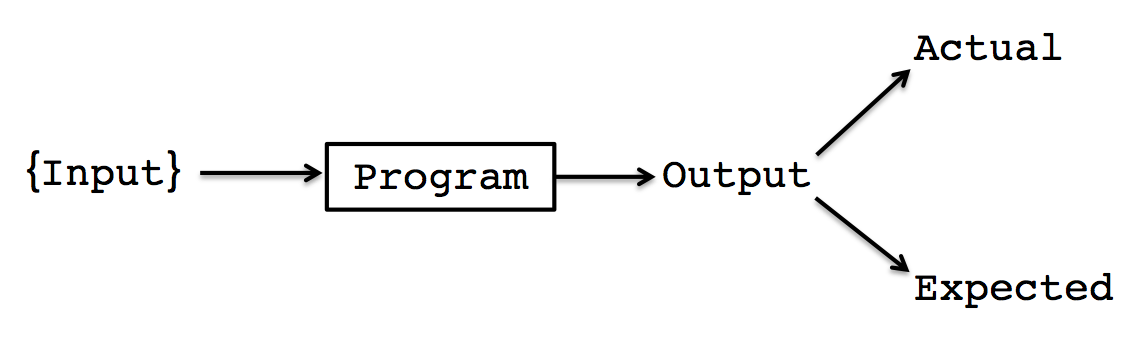
\includegraphics[width=90mm,scale=0.5]{diagram.png}
\caption{Basic Workflow of a software program}
\label{fig:workflow}
\end{wrapfigure}
Then, she must know how to read or understand the actual result and be able to compare it to the expected.\footnote{Consequently, many companies often build the role of tester into the role of developer, since the developer has the most intimate knowledge of the design and implementation of the software, and therefore has a better sense of what the output of the program exhibits. Even then, it may be impossible to describe the ideal expected output of the program.} In immensely complex scientific software or finanical programs swathed in accounting terms, the output of the program might be an unknown language to the tester. Even if the tester is a domain scientist, the output may be too complicated to read quickly and identify the trends that indicate she received a postive test result.

Another major challenge in software testing is the need to know all the possible situations one may want to test for. In an automobile simulator, for example, a tester does not want to just test for braking and accelerating, she wants to test turn-signaling, beeping, and brake-lighting, and also combinations of those tests to make sure that the beeping sensor does not accidentally disable the brake pedal capability. Knowing and describing every single situation may be unknown to the tester; they may not even think that that is a situation they have to test for. But these situations must be tested. What is known as the ``happy path'', the operational choice that most frequently represents the typical testing scenario, is certainly necessary for testing the program’s reliability, but it does not find the bugs. Outlier situations find the bugs. Lindvall et. al summarize the need for edge cases in their research in testing autonomous drones: ``Just because the drone behaves in a safe manner for a set of test scenarios does not mean that it will always behave in a safe manner for other scenarios''~\cite{Lindvall:2017:MMT:3103620.3103632}. Identifying all these possible outlier situations is \textbf{Problem One}.

With human's prolific ability to create and store data quantifying the world around them, it is hard to imagine that a tester could not find data that they could use. Gotterbarn agrees that ``Insufficient data is not a problem''~\cite{Gotterbarn:2016:CFC:2874239.2874248}. For example, consider an ocean temperature monitoring software that has predictive power in future local hot spots or cold zones. Ocean temperature data points do exist, and the missing points can likely be interpolated quite easily. But this is a sample size of one. To be sure the temperature projection software is robust, the tester would want to study a variety of circumstances and possibilities – situations that do not even exist. They might perhaps want to study temperature diffusion trends as a result of a hypothetical significant event 30 years from now. Data for that particular test case has to be created.

This is \textbf{Problem Two} -- writing the actual test data itself. A symbolic description of the test must be turned into an actual concrete input to the software. A test vector checking that beeping does not disable braking must be turned into ``beeping=5s\&\&braking=true'' or whatever discrete format the SUT requires. This is not a step that should be done manually. For example, VisIt, a graphical visualization tool, is capable of handling several gigabyte files~\cite{VisIt}. No tester wants to or even could write three gigabytes of data points modeling a real-world situation by hand just to satisfy one test case. Nearly every software testing paper agrees that writing data by hand seriously hinders the testing process~\cite{Misailovic:2007:PTG:1287624.1287645,Murphy:2007:PRT:1292414.1292425,Palka:2011:TOC:1982595.1982615,Patrick:2016:ATI:2970276.2970333}.

It is significantly easier to describe the trend of a certain test than it is to create the hundreds (if not more) data points that fit that description. Therefore, the goal of this project is to bridge that gap. It aims to aid the tester in designing and creating test suites so as to provide automation in the testing process. Automation, simplicity, and ease of use are key tenets of this project. Making a tester's job easier is much more likely to help them do it well, and making this tool accessible and easy to use is a low-cost, high-convenience solution that not only codifies a standardized testing procedure but shortens the duration of the testing phase and ensures resilient software before its deployment date. 

\chapter{\normalsize Literature Survey}
%literature survey
One key problem of software testing is knowing what to expect in the output of any given program. The essence of the oracle problem is best captured in the definition of non-testable programs, provided by Weyuker:
\begin{quote}
A program should be considered non-testable [if] (1) there does not exist an oracle; (2) it is theoretically possible, but practically too difficult to determine the correct output~\cite{Chays:2000:FTD:347636.348954}
\end{quote}
There are a variety of reasons why the oracle does not exist or cannot be exercised in a practical capacity. Weyuker describes that some software systems are like magic calculators – they are meant to inform us of the answer. She additionally mentions that some programs produce output that is impossible to read, either because of its volume or complexity. Here lies the core of software testing challenges. It is impossible to solve for every oracle or be able to describe every detail of a complex oracle – every system is entirely different. It goes without saying that this is even more impossible when there are time and resource constraints on the software development timeline. Consequently, a number of researchers have attempted to automate the creation of oracles~\cite{6963470}. For example, one research group used natural-language processing techniques to extract Java comments and design test cases that generate exceptions~\cite{Goffi:2016:AGO:2931037.2931061}. Another group identified and compared outputs of redundancies in software, using them as pseudo-oracles~\cite{Carzaniga:2014:COI:2568225.2568287}. However, the problem of generating complete, automatic oracles remains unsolved. While my project will not make any attempt to create oracles, it will provide information about the input. The test data will be constructed backwards in a sense. Instead of creating random data and then trying to discover its patterns, I will describe a trend and create data that fits that trend, in the hopes that knowing the input's shape will give meaning to the expected output.

Some researchers have done away almost entirely with creating oracles by developing techniques specifically used on non-testable programs~\cite{Lindvall:2017:MMT:3103620.3103632,Segura:2017:TAD:3103620.3103626,Chen:2015:MTS:2819261.2819278,Chen:2016:SOC:2970276.2970366,Lindvall:2015:MMT:2819009.2819030}. Metamorphic testing exploits the relationships of different executions of different input data. For example, upon white box inspection of a system, testers can see that outputs should relate directly to their inputs. They may not know much else about the system, or what its output means, but they know what differences they should see upon two different executions. Upon a certain execution they get f(5) = 20, and since they know the input-output relates directly, then they should predict that f(6) $>$ f(5). 

Other researchers have proposed methods that do not attempt to provide or calculate an oracle, but rather aid the tester, informed of the structure of the system, exactly what details she should watch and constrain about the oracle~\cite{Patrick:2016:ATI:2970276.2970333,Souza:2016:SMT:2897010.2897012,Harman:2011:SHO:2025113.2025144,Staats:2012:AOC:2337223.2337326}. The idea is that if an existing test suite can find artifical bugs in a system, it not only can find real bugs but also inform the tester what parts of the code must be correct in order for the system not to fail. This approach is called mutation testing. When a test suite finds artifical bugs, it determines which variables in a system are most effective in revealing faults, and then present them to the tester to manually define. This makes the construction of an oracle quite a bit easier.

The problem with metamorphic and mutation testing is that, while they skirt automatic creation of an oracle, they require just as much effort to develop as just creating an oracle by hand. Discovering metamorphic relationships requires a high level of implementation knowledge to write. Mutation testing requires a substantial amount of setup work, and still turns to the tester for manually defined expected values. Even though these techniques are considered cutting-edge testing methods, they do not provide any automation and therefore are not usable enough.

The need for automation is why random testing has developed such popularity. Random testing is not new, but it also is not very useful. Neither \textit{purely} random testing nor purely random data generation is strong enough to adequately test all branches of the code, nor does it provide any useful information about the test case itself or the data it contains. Consequently, constrained randomness, or using randomness in conjunction with other techniques, has gained the benefits of randomness' automation with the structure of other established testing methodologies.

The biggest complaint of pure random testing is that of the distribution type typically implemented: uniform distribution, which is why Lu recommends sampling along sample-space partitions non-uniformly~\cite{Lu:2018:URS:3184558.3186240}, preferring uneven numbers of ``Random Node'' selections and ``Random Edge'' selections. Another generalized technique is that of continous feedback. Arcuri describes Adaptive Random Testing, which monitors the success of the result of a random test case, and then appropriately chooses the next input to be unlike the previous input to attempt to trigger a different result~\cite{Arcuri:2011:ART:2001420.2001452}. All input choices are random, but directed towards certain trends. Arcuri identified a primary problem with this technique in that it often finds repeat bugs and does not extend to as many situations that pure random test cases otherwise could have found. However, several recent  groups similarly use a continuous feedback loops to identify the next test cases but with greater control over random stepping so as to address Arcuri's concerns~\cite{Yatoh:2015:FRT:2771783.2771805,Hughes:2016:FMB:2896921.2896928,Sabor:2015:ART:2819261.2819271}. Finally, one group used random grammar derivations limited to a finite size to generate programs to test compilers~\cite{Palka:2011:TOC:1982595.1982615}. Again this harnesses the automation of random while limiting its recklessness with additional constraints that guide the random selection.

Applying constraints on random data generation is particularly topical to areas of Machine Learning and Database-Driven applications. A team from Columbia University constructed a framework for generating test data for machine-learning models that produce ranking decisions on likely failability of a network of devices. Not only did their framework take in to account the number of examples and number of attributes of a dataset, it considered appearance of repeat values, missing entries, and partitioned categories of examples~\cite{Murphy:2007:PRT:1292414.1292425,Murphy:Kaiser}. However their tool only implemented uniform distribution and could only produce positive integers. This is a keystone feature that indicates the specialization of their framework, and makes extensibility to other applications of software testing nonexistent without significant refactoring. In regards to database-driven applications, there is a considerable lack of developing in testing. The typical approach of data generation is really quite limited in its power. That data really only passes synactic checks, like matching database schema descriptions, and general ``not null, unique, primary, and foreign key constraints''~\cite{Haller:2010:TDC:1838126.1838132}, which indicates that the links between data tables makes sense. The data is database-compliant, it does not have any mistakes, but it contains no semantic meaning. It does not exhibit any trends or patterns. The shortcomings of these applications influence the desired features of my project.


\chapter{\normalsize Proprosed Argument}
%proprosed argument
I believe that I have designed an approach to these problems and have architected a simplistic solution that automates the steps described in the introduction. I hypothesize that Problem One is solved by the advent of combinatorial testing, which identifies most, if not all, of the test cases necessary for confidence in working software. My tool, Parmgen, has solved the second problem, translating the English description of a test case into a concrete format that can be used as input into the program. I ask the user for smaller, more simplistic descriptions of their input data, which requires less work than writing every data point by hand. Then I can use Python's random statistical distributions to generate those points and write them to a convenient location for the tester’s use. This tool is written in the Python language, which is useful for prototyping the MVP (Minimum Viable Product) of this tool. I call this entire pipeline GenSequence.

\chapter{\normalsize Background on Design Decisions}
%background
\section{Parameters}
The ``input'' to a program is a set of parameters, named variables that represent specific groups of data points. How those parameters are generated, and what literal form they take, effects the outcome of the program. Large programs with larger inputs may benefit from having their input parameter data sets generated by statistical distributions.

I was inspired to create this tool by testing a project I helped build in my software engineering class, which took in the records of each student in a class of 40 students, describing things like their skills in certain technologies and their available free times during the week. This project made a fairly sophisticated decision about how to form optimal groups of students to work in teams, ensuring that each group has complementary skills and overlapping free times. During testing, it is important to consider bizarre scenarios, like what should happen when no student has any free time at all, or when half the class can only meet early in the week and the other half can only meet late in the week.

These parameters can follow certain trends that can be mimicked by repeated trials of statistical distributions. The input to this program is merely an Excel csv file of a record table, such that every row is a student's entry and every column is all the entries for a certain parameter that really effects the outcome of the program. Figure \ref{fig:teamfile} shows the CSV file of the literal input into the Team Building program. The software takes in the filename, opens the file, and parses the data. Each row is a student, and each column is a parameter, such as free time availability on Monday or self-rated HTML experience level.

\begin{figure}
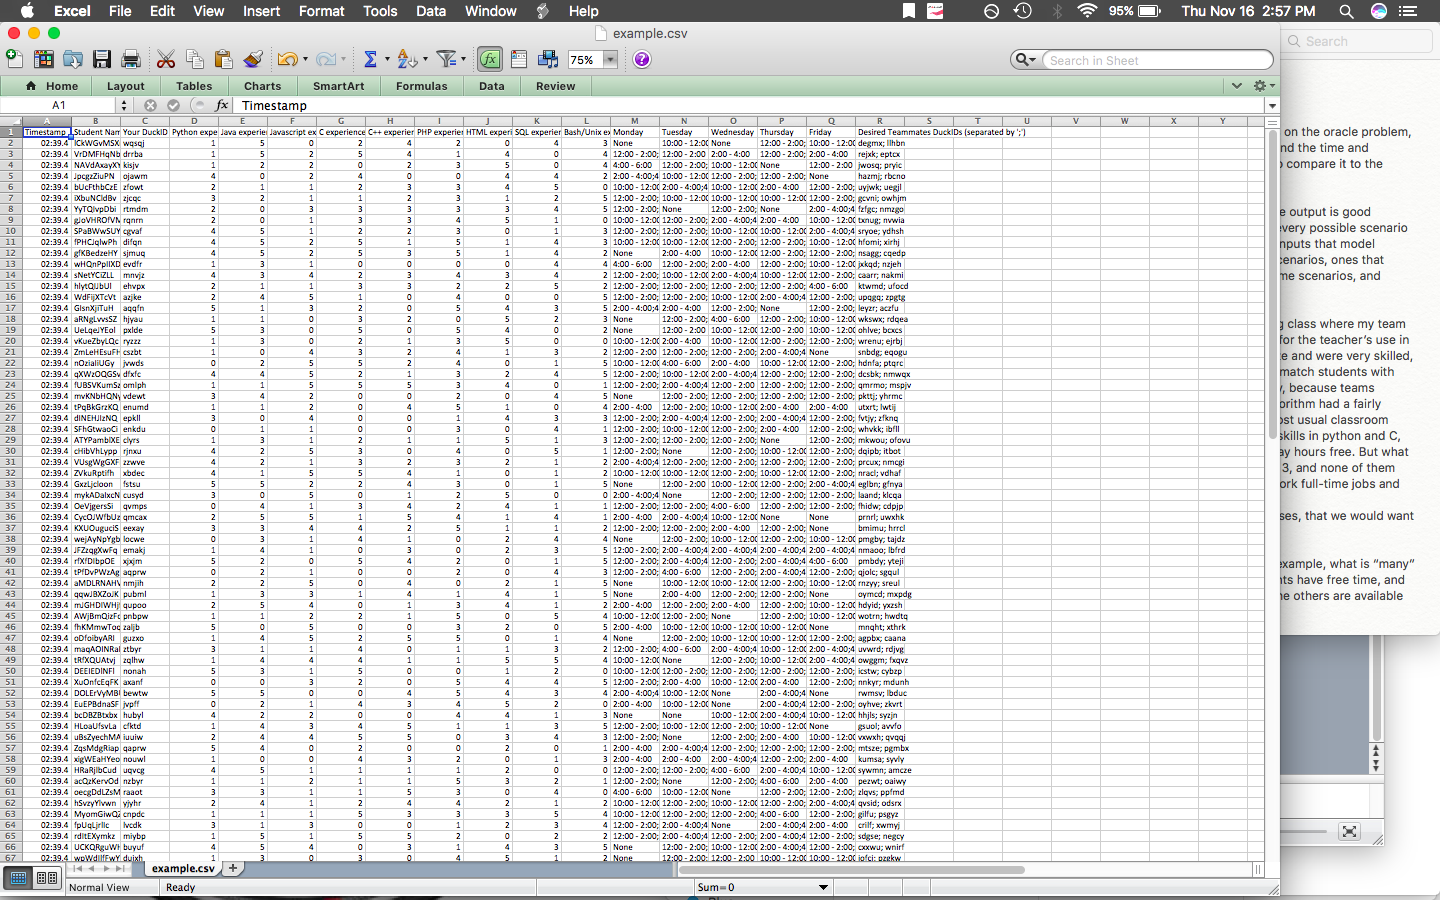
\includegraphics[scale=0.3]{team-file.png}
\caption{A CSV file of a test case input into the Team Builder program}
\label{fig:teamfile}
\end{figure}

\section{Pairwise Testing}
GenPairs is a pairwise testing tool~\cite{Gen:Pairs} that creates symbolic test vectors that describe what each test case should generally look like, using English adjectives to describe what the input should be. Pairwise testing rests on the hypothesis that a majority of faults in a program are a result of combinations of parameters that work with one another to create or amplify a problem. Creating the minimum number of test cases that satisfactorily describe all combinations of possible parameters gives the maximum code coverage. The success of finding all faults increase with greater numbers of combinations of parameters; that is to say that all combinations of four parameters will find more faults than all combinations of three. However, pairwise testing finds all combinations of two parameters and is often sufficient for maximum code coverage while still reducing the time, and therefore cost, of creating or running all test cases. This is even more likely when the total number of parameters is also somewhat low. Combining only two parameters is a matter of convenience and time, since more test cases require more time to create.

While translating a symbolic test vector to concrete data may present a challenge, it is extremely valuable in reducing the uncertainty of knowing what sort of trend the input test data follows. Say, for example, a tester needs to generate a concrete point for this test vector (Table \ref{table:testv})

\begin{table}[h!]
\centering
\begin{tabular}{@{} *5l @{}}    \toprule
\emph{Item Purchased} & \emph{Price} & \emph{Delivery Method}  \\\midrule
Large Item & Expensive & Ultrafast \\\bottomrule
 \hline
\end{tabular}
\caption{Single Symbolic Test Vector}
\label{table:testv}
\end{table}

She knows that some test case will send a large item by ultrafast means. In our generation of concrete data (described in the next section) in this test vector, she might come across the test case in Table \ref{table:conctc}

\begin{table}[h!]
\centering
\begin{tabular}{@{} *5l @{}}    \toprule
Motorboat & 18700.00 & Jet Airplane \\\bottomrule
 \hline
\end{tabular}
\caption{Single Concrete Test Case}
\label{table:conctc}
\end{table}

The interaction of these two parameters, a very large object sent by ultrafast means, ought to trigger a bug in the system, because perhaps her company does not have that capability. If this situation is not handled correctly in the software, the user of the software, the customer, will be misled about the quality of their shipping network. This example is very trivial, but it exemplifies the problem well, and shows how pairwise testing methods can bring this awareness to the tester and developer and help them improve their software. Now imagine a much longer and complicated test vector in a very advanced version of the company’s ecommerce website; maybe now it has millions of possible item categories and hundreds of shipping methods and can also handle coupon codes and student discounts and special offerings: many more parameters to consider. It is helpful to know that the test vector was created from a description including Large Item - Expensive - Ultrafast. The symbolic test vector describes the input well enough for the tester to understand and use common sense to predict what the output ought to be. Then if she tests that test case and finds that the customer receives a message that sending a boat through lightning speed mail is impossible, she gains more confidence that her program works correctly.

The pairwise testing tool is designed such that the tester describes all the possibilities for what each parameter could possibly be, and then the tool generates all the test vectors that describe what the parameter ends up becoming. When using this tool, testers should list every kind of statistical distribution that they would be interested in seeing, or what makes sense in the context of their program. This is so important because it makes GenSequence a more applicable tool for database-driven applications. If a tester would benefit from giving meaning to the data trend, they can benefit from using the GenSequence framework. This is the semantic sense that is often missing in testing database programs.

Most importantly, Pairwise testing satisfies the need to test ``outlier'' cases. The very function of pairwise testing ensures that a combination of classifications of parameters occurs at least once in the test suite. This is a test case that the tester might have otherwise forgotten or overlooked. It guarantees robust testing.

\section{Context-Free Grammars}
We can use the ideas of context-free grammar derivations to generate concrete test data. We call this feature Makogram, a tool implemented in the Python templating tool Mako~\cite{Mako:Template}. Say a test case has the following production rule:

\begin{grammar}
<Case> ::= <Item> <Price> <Delivery Method>
\end{grammar}

What constitutes an item? Item might have a production rule

\begin{grammar}
<Item> ::= `Ship' | `Book' | `Loaf'
\end{grammar}

The grammar tool used is constructed such that a non-terminal can be the result of a function, and that result can be a randomly generated data point. For example,

\begin{grammar}
<Price> ::= fun \{ random_choice(8,15) \} ( )
\end{grammar}

Meaning that the data point for the Price parameter would be some number chosen at equal randomness from any number between 8 and 15.

A terminal symbol can be written to be the returned result of a much more sophisticated function - one perhaps that returns a Gaussian distribution of data points. For example, consider an earthquake modeling program, which takes a set of data points for its magnitudes parameter, and it can have all sort of descriptions attached to it: Gaussian, uniform, cardioid, etc. All of these descriptions will occur somewhere in a test vector, so each is mapped to the corresponding function. When the magnitudes parameter is set to be generated from a bell-curve distribution, the bell-curve random generator will generate that set of points.

Generating good test data for actual magnitudes of an earthquake must be based on the knowledge that a magnitude cannot be negative or greater than 10.0. This is the limit of the program. It cannot make logical guesses about the natural language of the parameter. But the tool is written to minimize the number of times the tester must identify this constraint –- just once, in the beginning.

Moreover, the power of grammars makes creating the data very easy. GenSequence provides support for the \textit{grammar} of the output csv files, which can be thought of as a template describing the ``language'' of a csv file. A derivation is a series of rule substitutions that eventually ends with a string. This ``string'' belongs to the language described by the grammar, and this string \textit{is} the test data that is usable for testers because the production rules gave functional data points. Makogram was constructed not just to limit the number of substitutions but to reach exactly the desired number. So if a tester asks for 30 examples (30 rows of data), Makogram will hand back exactly 30 rows.

\section{Law of Large Numbers}
The Law of Large Numbers states that the actual outcomes will approach the expected outcomes as the sample size increases to infinity . One canonical example is a series of coin flips, with an equal probability of flipping heads as tails. It is expected that exactly 50\% of the samples will be heads and 50\% tails. In a sample size of only one hundred flips, the percentage of heads to tails may only be 46.0\% - 54.0\%, but a sample size of ten thousand would come far closer to an even 50-50 split, possibly 50.37\% - 49.63\%. 

This principle applies to all kinds of probability distribution types, not just coin flip probability. Students’ grades tend to figure towards a bell-curve distribution, but a graph of 50 students’ grades will look more misshapen than a graph of thousands of students’ grades. Moreover, the principle applies to many programming languages’ utilities that support randomness. The Python language contains a built-in module called random which provides a variety of generators for all flavors of probability distribution. Individual points are generated according to a particular distribution, and the generation of a large enough sample size is guaranteed to follow the expected trend.

How large is large? Bernoulli proved that the actual outcome of a simulation would approach the expected outcome as the sample size grows to infinity. So in general, the greater the sample size the more accurate the results.

If the use case arrives on the order of hundreds of data points, a default sampling size on the order of ten thousand randomly generated data points should suffice. Because the initially generated set of points is far too many, I have devised a scheme to reduce the sample set to the appropriate size while still encapsulating the distributions guaranteed by the Law of Large Numbers. For each parameter, I generate the too-large sample size, sort it in increasing order, and selectively choose every nth point to include in the reduced set of points, such that the size of the reduced set is the desired number –-  however many the test case needs.\footnote{Given the statements of the previous section, some clarification is in order. Context-free grammars would imply that the random function would be called upon every derivation of a data point. But since the number of derivations is limited, that would mean that the number of function calls would be minimized, which would not produce the desired distribution. GenSequence declares the grammar, and then uses what I call a Parm object to create a large sample size and reduce it down into a small pool. When a derivation of the grammar is instantiated, it calls upon the pool, which yields singular points.}

I have yet to rigorously prove this selection scheme, but I hypothesize that it suffices for now, and does indeed capture the essence of the Law of Large Numbers. Pictorial representations show that this paradigm is not perfect, but is certainly far better than choosing exactly the desired number of points. Visibly a sample size of 300 systematically chosen from a large set follows the curve of 10,000 points much more closely than 100 initial points.

\begin{figure}[H]
\centering
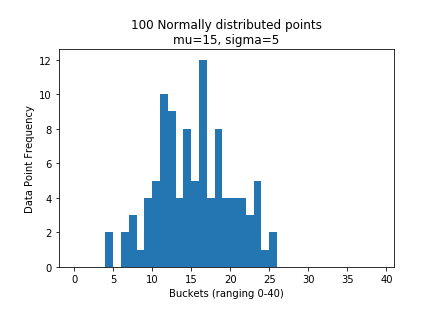
\includegraphics[scale=0.7]{law1.png}
\caption{Histogram of point values generated by normal distribution - sample size 100}
\label{fig:law1}
\end{figure}

\begin{figure}[H]
\centering
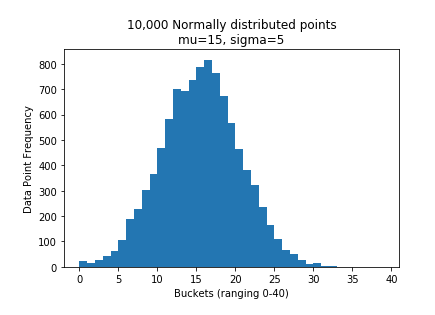
\includegraphics[scale=0.7]{law2.png}
\caption{Histogram of point values generated by normal distribution - sample size 10,000}
\label{fig:law2}
\end{figure}

\begin{figure}[H]
\centering
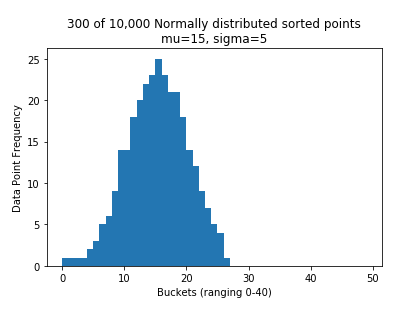
\includegraphics[scale=0.7]{law3.png}
\caption{Histogram of point values generated by normal distribution and reduced to sample size of 300}
\label{fig:law3}
\end{figure}


\section{Cardioids}

In some testing situations, it may be useful to consider the relationship between two parameters, a relationship that mimics real life. For example, a physics-modeling simulation might have a loose property that larger objects move slower than smaller objects. These two parameters, size and velocity, are interdependent.

A Cardioid\footnote{The name cardioid was chosen for its polarity. Its figure encompasses an area such that a majority of the space (about 90\%) sits on one side of an axis and a small section (about 10\%) sits on the other.} object acts as a two-column parameter. The end user specifies the relationship between the two sub-parameters by providing descriptions of what data point range pairings are preferred (called favorites) and what data point range pairings should only occur infrequently (called outliers or non-favorites). The data generation step will look at these descriptions and generate the data point pairings such that 90\% of the samples are favorites and 10\% are outliers. For example, the tester will specify favorites for the cardioid relationship between size and velocity: large and slow, medium and medium, and small and fast. Non-favorites are outlying particles: small and slow, and large and fast.

The cardioid relationship spanning two parameters occurs only if the tester specifies it as a possibility in the test vector creation step. There are certainly situations where it does not make semantic sense to use cardioid relationships. It does, however, allow testers to generate tests that maintain realistic sense. It also allows the user to include their own test data generation constraints if statistical randomness does not quite suffice.

\section{Preprocessing}

An important arm of the automation pipeline is developing a baby-sized language that is easy to write yet fully describes everything a tester wants out of this tool. Then a preprocessor can read this language and generate the code that, when executed, will create the data. Writing the data-generating code itself is complex enough that it limits automation, and building a machine that performs this step systematically significantly increases ease of use. I have fully developed the language into basic syntax and grammar rules, which the tester can then write in a .prm file.

I have also constructed a simple preprocessor to parse this information. It is very lightweight in that it compiles quickly, but does not have advanced error handling or give helpful compiler errors. The current iteration implements Ply (Python Lex-Yacc)~\cite{PythonLexYacc}. Ply works in two general steps. First it reads the input and identifies characters or words into tokens –- essentially describing the type of each word or character. This is the lexing, or ``tokenizing'', step. Next, the parsing step, parses the tokens altogether by identifying the grammar rules that combine them. Once the information has been identified as a derivation of a grammar rule, it is then available for interpretation. The preprocessor does not yet use Ply to read the entire .prm file, and mostly uses Python file-processing techniques, but the language is simple enough that I had little difficulty rendering the information into the data generator. For an MVP this tactic suffices.


\chapter{\normalsize Methods}
%methods

One key part of this project is deciding if it accomplished its goal and answered its research questions. 
\begin{enumerate}
\item Is using random statistical distributions a valid approach to writing test data?
\item Do symbolic test vectors provide enough information about the input that it informs expectations of the output?
\item Does GenSequence make a tester's job easier or save her time?
\end{enumerate}

GenSequence's intended use is for new projects, pieces of software that do not already have a monolithic code base. However, testers might use this tool at any stage during the software development cycle if they lack a substantial test suite. Perhaps their application is highly advanced, has been neatly designed, and has fixed bugs found through other means of testing or from end user reports. Therefore, that piece of software simply may be bug--free. That is unlikely, but it is possible. So measuring the usefulness of GenSequence on fault finding ability alone would depend on the state of the software it is testing, giving the indication that GenSequence is inadequate when really the software is just really well done.

It is important to determine how valid the random statistical distribution approach is. I will use a few case studies to determine if knowing how a parameterss data was generated helps clarify the expected result. First I will test my testing tool against a planetary orbits simulation. Then I will observe my tool's data representation in an earthquake analysis program. 

In response to both Question 2 \& 3, the intention of this project was to streamline the testing process, and provided automated methods of data creation. The usefulness of this program is measured by the ease of test suite creation. I will consider these general metrics: the length of the script generating data, how much code a tester would have to write, and how quickly the data is generated (more data takes more time). If it is easier for a tester to write a GenSequence spec than to write a full test suite by hand, then GenSequence is a valuable tool, and it might encourage developers to write more thorough test suites.

Ultimately it is a tester's decision as to how useful this project is. More features added to the project only increase the ease of use, since a machine does more of the heavy lifting than a human brain and body otherwise would have. However, it is only useful when a test suite does not exist or in circumstances when it would be easier to generate a test suite by hand. There is further discussion later.

\chapter{\normalsize Results}
%results
\section{Celestial Body Simulation}
Initial use of GenSequence on the planetary orbits program proved some promise in the capability of this tool. I used the tool to generate 30 test cases. Test case 13 was programmatically named:
\vspace{1cm}

\noindent\fbox{
    \parbox{\textwidth}{
        {\fontfamily{pcr}\selectfont
        13-70-mass|right_slanted-position|right_slanted-velocity|uniform-diameter|left_slanted.csv
        }
    }
}

\vspace{1cm}
13 describes the test case number, 70 describes the number of rows in the test case. In this simulation, each row represents an instance of a planetary body.

Planetary masses were generated with a right slanted distribution. Position, the location of each body, was generated with a right-slanted triangular probability. The velocities of the bodies were generated uniformly. The diameters, the visible size in the program's GUI, were generated by a left-slanted distribution. The starting point of this program's test data showed this visualization:

\begin{figure}[h!]
\centering
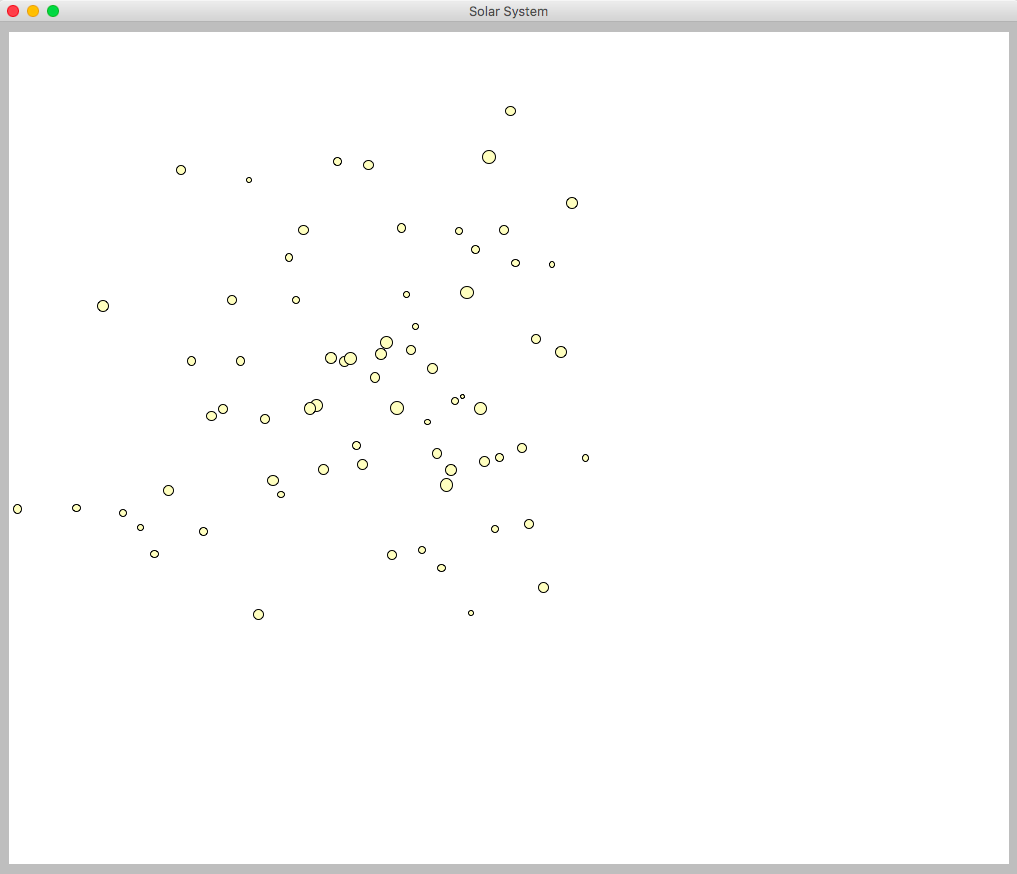
\includegraphics[scale=0.4]{start-ex.png}
\caption{Starting Locations of 70 celestial bodies}
\label{fig:startbody}
\end{figure}

Figure \ref{fig:startbody} accurately reflects the visible parameters – position and diameter. The positions were generated by a right slant, and ostensibly so, the bodies are mostly located in one region. The diameters were generated by a left-slanted distribution, clearly slanted towards a smaller diameter, with most samples appearing small or medium size, but a notable number appearing fairly large.

The program by nature tracks and draws the motion of each planetary body through time, giving a useful summary of the program’s execution by the end of the simulation (665 time steps). Running test case 13 garnered Figure \ref{fig:endbody}.

\begin{figure}[h!]
\centering
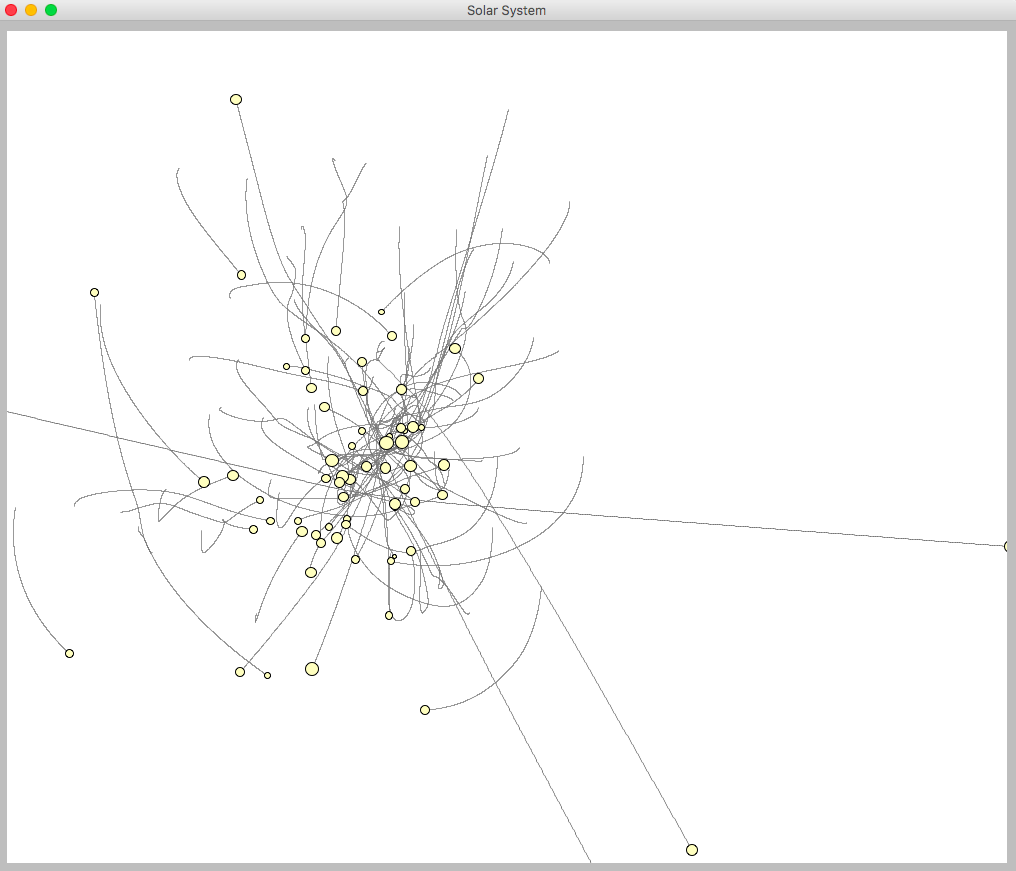
\includegraphics[scale=0.4]{final-ex.png}
\caption{Ending Locations of 70 celestial bodies after 665 time steps}
\label{fig:endbody}
\end{figure}

Spending a minute closely observing these paths registers some important observations about the natural behavior of gravity acting on planetary bodies. Some disobeyed their trajectory and were redirected by the large mass in the center. The initial velocities manifested themselves as well. The paths are of all different lengths, which makes sense since they were generated by a uniform distribution.

\section{Earthquake Analysis and Visualization Program}
The earthquake analysis program performs basic statistical analysis of magnitudes, locations, and depths on a map, and also plots quake events on a map. Bigger dots represent a greater data point value (This is important to note because dots representing magnitudes describe their intensity not their destruction coverage). One test case had a file name (test vector) of:
\vspace{1cm}

\noindent\fbox{%
    \parbox{\textwidth}{%
        {\fontfamily{pcr}\selectfont
        6-70-magnitudes|cardioid-latitudes|left_slanted-longitudes|right_slanted-depths|cardioid.csv
        }
    }%
}

\vspace{1cm}
Observing the cardioid relationship between latitudes and longitudes is confirmation of GenSequence working. GenSequence was programmed with the following information:
\vspace{1cm}

\begin{lstlisting}
#magnitudes ranges
Micro = Range(0.0, 2.0, exclusive_upper=True)
Feelable = Range(4.5, 7.9, exclusive_lower=True)
Great = Range(8.0, 9.5, exclusive_lower=True, exclusive_upper=True)
#depths ranges
Shallow = Range(0.0, 5.0, exclusive_lower=True, exclusive_upper=True)
Mid = Range(5.0, 15.0)
Deep = Range(15.0, 30.0, exclusive_lower=True)
...
# specify the relationship between magnitudes and depths
MagsDepths = Cardioid(Mags, Depths)
MagsDepths.setFavorites([(Micro,Shallow), (Great,Deep), (Feelable,Mid)])
MagsDepths.setNonFavorites([(Micro,Deep), (Great,Shallow), (Feelable,Deep), (Feelable,Shallow)])
\end{lstlisting}

\vspace{1cm}
This is the literal implementation of the tool describing the most frequently occurring data pairs in this test case. Low intensity magnitudes should be near Earth’s surface and very intense magnitudes should occur deep below the earth’s surface. Moreover, it is not very frequent that low-intensity earthquakes occur very deeply, and high-intensity earthquakes occur very near surface. \footnote{This assumption may be entirely false about the nature of earthquakes. This trend is one I invented to add functionality to GenSequence, one that could easily be reversed by any seismologist user of the program.}

The plots of magnitudes and depths (Figure \ref{fig:magsdepths}) show this constraint propagating:
\begin{figure}[h!]
  \centering
  \begin{subfigure}[b]{0.6\linewidth}
    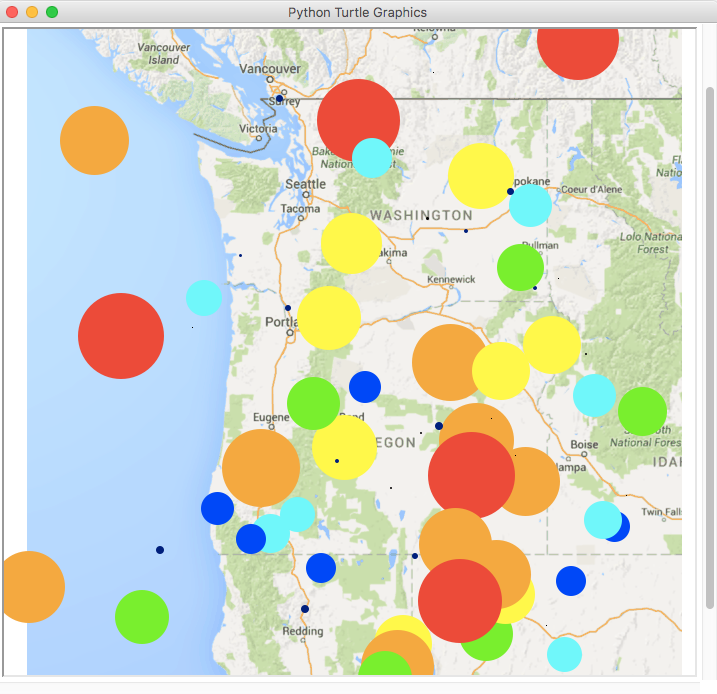
\includegraphics[width=\linewidth]{mags.png}
    \caption{Magnitudes}
  \end{subfigure}
  \begin{subfigure}[b]{0.6\linewidth}
    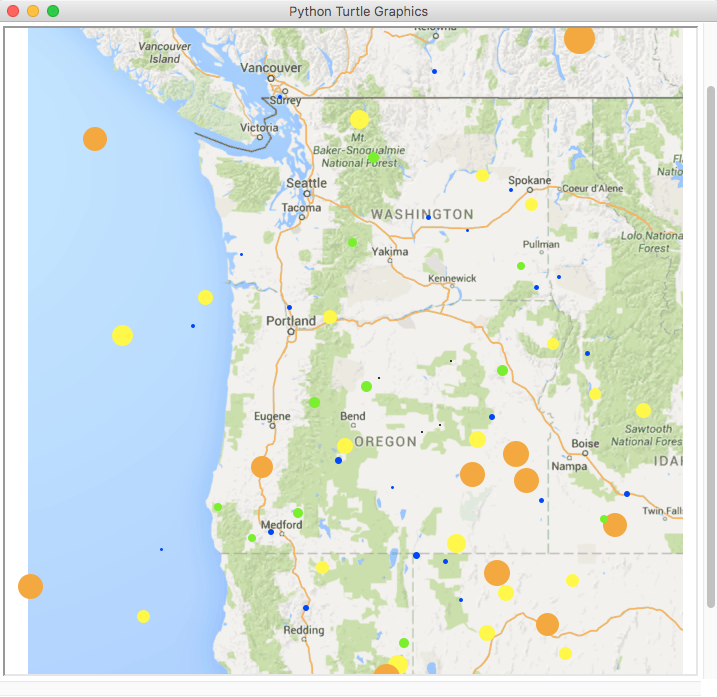
\includegraphics[width=\linewidth]{depths.png}
    \caption{Depths}
  \end{subfigure}
  \caption{Plotting Magnitudes and Depths from the same test case}
  \label{fig:magsdepths}
\end{figure}

The correlation is rather difficult to piece but does reflect exactly what is expected. The large red dot due west of Portland has a matching yellow depth dot. The small blue event due west of the Oregon-California border has a matching blue dot in the same place. One outlier is a sizable orange earthquake covering the Umatilla forest that has a very tiny blue depth dot.

Considering latitude-longitude oriented north-up, west-left, east-right, south-down, and given the left-slanted-ness of the latitudes and right-slanted-ness of longitudes, this test case should mark the locations of the earthquakes mostly drifting towards the lower-right corner. This is in fact what the program generates (Figure \ref{fig:clusters}).

\begin{figure}
\centering
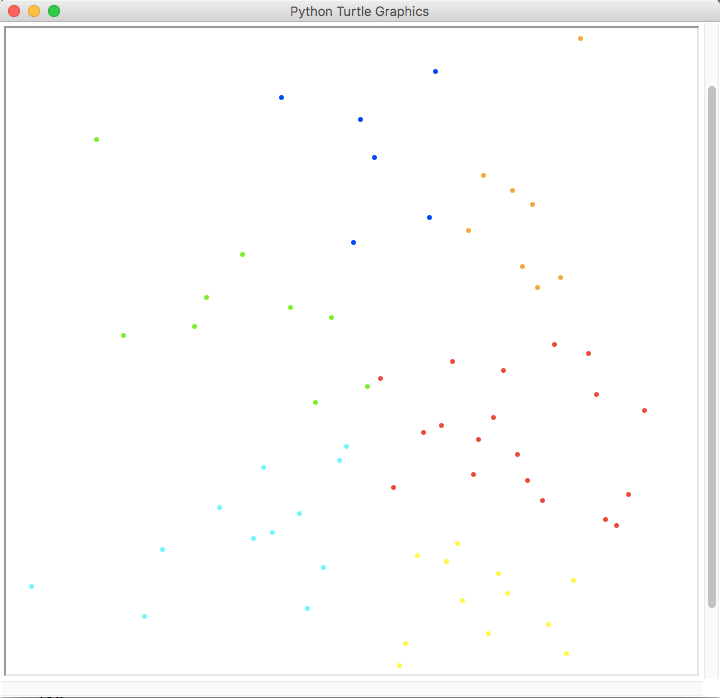
\includegraphics[scale=0.5]{clusters-nobg.png}
\caption{K-Means Clustering of Earthquake events from case 13}
\label{fig:clusters}
\end{figure}

\chapter{\normalsize Concluding Thoughts}
%conclusion

I believe that GenSequence's best application is for testing database-driven applications. These applications literally control the world. Consider financial applications alone: the record of every transaction, every payment, every credit report, and every bill can dictate a person’s entire life. The infrastructure surrounding that data must not expunge or fabricate any of it, and must maintain its integrity. Software that accesses, controls, and manipulates this huge amount of data carries substantial responsibility. Moreover, software that can read, interpret, and identify trends in a huge wealth of global data has amazing power in informing us of what happens in the world and how we can make better decisions. It is therefore of utmost importance to design that software well enough to trust its results.

GenSequence has addressed those demands. It functions simply but provides automation during the testing stage and generates reliable data that is what is says it is. If the context of the program warrants consideration of statistically unlikely but possible scenarios, GenSequence can make that happen. It primarily states its power by its ease of use and nearly end-to-end automation. Moreover, the construction of data points does provide insight into the expected output. However, this insight is limited to eyeballing the result.

Given that the construction of GenSequence was a Minimum Viable Product, there is considerable room for improvement. What follows is a discussion of future work and extensibility.

\textbf{Current Iteration}
\begin{itemize}
\item Identify an open-source project in need of a test suite, and create a hypothetical test suite for it using GenSequence. The greatest indication that GenSequence is useful is cross-checking it against a program that someone else wrote.
\end{itemize}

\textbf{Top of the Backlog}
\begin{itemize}
\item Implement the entire preprocessor in Ply, develop an abstraction for a model of the Parms, and develop an interpreter that could execute those models. Currently the preprocessor performs most of its parsing via line-by-line file processing, which is an inelegant and clunky solution.
\item Combine the specifications that enter GenPairs and the preprocessor into one; in other words, combine the roles of the .cp and .prm files. This would certainly reduce the work for the tester. In initial design of the prm language I had included distribution possibilities for each parm, but had removed it from prm since it was already specified in cp language that went into GenPairs. Ideally this specification could be parsed and found from the prm file and automatically sent into pairwise generation.
\item Develop greater control over Double cardioids - relating multicolumns together. I had this idea when developing data for TeamBuilder. I wanted control over the relationship between general skills (columns Python and Java) and more niche, specialized skills (like Haskell and C pthreads library). This required generation of two cardioids, and then calculation to determine what pattern each data instance matched, and then resorting by implementing a hill-climbing technique. This quickly fell out favor, as much more of the system needed implementation first.
\end{itemize}

\textbf{Icebox}
\begin{itemize}
\item Consider alternate formats for the output. Currently GenSequence will give the tester a csv file of raw data. However in database-driven applications, the test data must come in scripts of database insert statements, as the database state must be restored for every test case. Consequently it is worth implementing a utility feature that outputs a database creation script, say for example a shell script containing SQL insert statements.
\item Rewrite usability documentation, and provide utilities that allow for easy initial use. Part of automation is that it is easy to set up, if even for a proof-of-concept.
\item Develop a greater understanding of how computer random works, and its influence on data generation according to distribution functions.
\item Research and identify possible Machine Learning applications in which GenSequence could be used. I believe that GenSequence might have applications in some ML models, in which case knowing the demands of ML models might influence the way GenSequence is used.
\end{itemize}



%\chapter{\normalsize This is the Title of the First Chapter}  % Use \\ for long titles %
%This is a sample document for the Auburn \LaTeX{} style-files known
%as {\tt aums} (for Master's papers) and {\tt auphd} (for Ph.D.'s).
%\begin{theorem} This is an example theorem.
%\end{theorem}%
%\section{This is an example of a section heading}%
%This is some text which follows the section heading. You can find the data in Table \ref{tab:results}.
%\begin{figure}
%  \begin{center}
%  \setlength{\unitlength}{.7in}
%    \begin{picture}(4.2,1)
%      \put(0.2,.5){\circle{0.1}}
%      \put(0.9,.5){\circle{0.2}}
%      \put(1.6,.5){\circle{0.3}}
%      \put(2.3,.5){\circle{0.4}}
%      \put(3.1,.5){\circle{0.5}}
%      \put(3.8,.5){\circle{0.6}}
%    \end{picture}
%  \end{center}
% \caption{Hollow circles 1}\label{HollowCircles}
%\end{figure}%
%\begin{figure}
%\centering
%  \begin{tikzpicture}
%\filldraw [double distance=0.20mm,very thick, fill=white, draw=black] (0cm,0cm) rectangle (5cm, 2.5cm);
%   \fill (2.5in,0in) circle (3pt);
%\end{tikzpicture}
%\caption{Some TikZ picture.}
%\end{figure}%
%\begin{table}[htb]
%\begin{center}
%\begin{tabular}{|c | c | c | c|}
%\hline
%\multicolumn{1}{|c|}{~} & \multicolumn{3}{c|}{Multicolumn Heading 1}\\
%Heading 1 & \multicolumn{1}{|c}{Heading 2} & \multicolumn{1}{c}{Heading 3} & \multicolumn{1}{c|}{Heading 4} \\
%\hline
%1 & 19, 20 (19.5)& NA & NA \\
%\hline
%3 & $\infty$* ($\infty$)& 18, 15 (16.5)& 9, 9 (9)\\
%\hline
%5 & 23, 18 (20.5) 
%& 16 (16)
%& 7, 7, 8 (7.33)\\
%\hline
%\multicolumn{4}{|c|}{*Some random comment for the whole table.}\\
%\hline
%\end{tabular}
%\end{center}
%\caption{Some Table of data}
%\label{tab:results}
%\end{table}%%

%\subsection{This is a subsection heading}%
%Text after the subsection. And we have a figure, Figure \ref{HollowCircles}.

%%%%%%%%Two options for having a bibliography. If you use a separate file or multiple files:
\bibliography{Phase2}
\bibliographystyle{plain}



\end{document}

